%% LyX 2.1.2.2 created this file.  For more info, see http://www.lyx.org/.
%% Do not edit unless you really know what you are doing.
\documentclass[12pt,english]{report}
\usepackage{mathptmx}
\renewcommand{\familydefault}{\rmdefault}
\usepackage[T1]{fontenc}
\usepackage[latin9]{inputenc}
\usepackage[a4paper]{geometry}
\geometry{verbose,tmargin=2cm,bmargin=2cm,lmargin=2cm,rmargin=2cm,headheight=1cm,headsep=1cm,footskip=1cm}
\setcounter{secnumdepth}{3}
\setcounter{tocdepth}{3}
\setlength{\parskip}{\medskipamount}
\setlength{\parindent}{0pt}
\usepackage{verbatim}
\usepackage{pdfpages}
\usepackage{graphicx}
\usepackage{setspace}
\usepackage[numbers]{natbib}
\usepackage{nomencl}
% the following is useful when we have the old nomencl.sty package
\providecommand{\printnomenclature}{\printglossary}
\providecommand{\makenomenclature}{\makeglossary}
\makenomenclature
\doublespacing

\makeatletter

%%%%%%%%%%%%%%%%%%%%%%%%%%%%%% LyX specific LaTeX commands.
\providecommand{\LyX}{L\kern-.1667em\lower.25em\hbox{Y}\kern-.125emX\@}
%% Because html converters don't know tabularnewline
\providecommand{\tabularnewline}{\\}
%% A simple dot to overcome graphicx limitations
\newcommand{\lyxdot}{.}


%%%%%%%%%%%%%%%%%%%%%%%%%%%%%% User specified LaTeX commands.
\usepackage{tauthesis}
\usepackage[font={small,bf}, labelfont={small,bf}, margin=1cm]{caption}
\usepackage{titlesec}
\newcommand{\hsp}{\hspace{20pt}}
\titleformat{\chapter}[hang]{\Huge\bfseries}{\thechapter\hsp}{0pt}{\Huge\bfseries}


\Title{\textbf{Kidney Segmentation and Renal Lesion Detection in 3D CT}}
\Author{\textbf{\large Neta Blau}}
\Year{October 2017}
\Supervisor{Prof. Nahum Kiryati}
\Department{School of Electrical and Electronic Engineering}
\Degree{Master of Science in Electrical and Electronic Engineering}
% \Degree{Doctor of Philosophy}

\makeatother

\usepackage{babel}
\begin{document}
\begin{comment}
This is Micheal JasonSmith's uocthesis example ported to \LyX{} by
Etienne Lalibert� (etiennlaliberte@gmail.com).

Alex Liberzon (alex.liberzon@gmail.com) modified it to the Tel Aviv
University format, with the header of the Faculty of Engineering.
You can open the tauthesis.sty to update it to your needs.

Go to \textsf{Document > Settings > \LaTeX{} preamble} to modify the
\textsf{Title, Author, Year, Supervisor, Department} fields.

Default processor is now PDFLATEX.
\end{comment}


\coverpage

\titlepage

\prelimpages

\begin{comment}
Split the thesis into separate chapters. Use \textbackslash{}include
mode to include the separate files.

Use \LyX{} Table of Contents, List of Figures, List of Tables and
Nomenclature automatics to include them in the thesis. Double - click
on each item to change the default level of contents, move the chapters
up/down and so on.
\end{comment}


\chapter*{Abstract}
Renal cysts are common in aging kidneys, and are usually found incidentally in patients undergoing abdominal imaging for other reasons. Although most cysts are benign, they require expert examination as some of them may either indicate the presence of a malignancy or evolve into one. So far, the proposed algorithms for the analysis and detection of renal cysts have been either semi-automatic or evaluated on fairly small data-sets. Here we present a fully automatic method to segment kidneys and to detect simple renal cysts. A fully convolutional neural network (FCN) is employed for segmentation of the kidneys. A combined 3D distance map of the kidneys and surrounding fluids provides initial candidates for cysts. Then, a convolutional neural network (CNN) classifies the candidates as cysts or non-cyst objects. Performance was evaluated on 52 randomly selected volumetric CT scans with more than 70 cysts annotated by an experienced radiologist, with promising results.

Another type of renal lesions are cancerous renal tumors. Though also usually an incidental finding, they are malignant and often fatal. Early detection of such tumors is highly advantageous for recovery. Using the same methods and similar data we attempted to develop a fully automatic system for detection of cancerous renal tumors. We present our experiments and preliminary results and discuss the steps we dim required to undertake this challenge.

\tableofcontents{}

\acknowledgments{I would like to thank my ...}

\textpages

\listoffigures


\listoftables


\printnomenclature{}


\chapter{Introduction}

% SKELETON: A (short?) paragraph to describe the importance of automatic diagnosis in medical imaging (reduce overload for radiologists, improve the chances for early detection of asymptomatic medical conditions, etc.) and the growing interest in such tools.
In a radiologist's line of work time is of the essence. The flux of imaging cases that require human attention is often overwhelming, forcing radiologists to increase their rate of diagnosis. This, in turn, inevitably reduces the quality of their work, causing some pathologies to go undetected or misrepresented. The consequences may vary between suboptimal treatment and considerable damage to patients' health. Automated tools that aid radiologists with their tasks are therefore highly desirable. %and can make the diagnostic process more consistent and complete%
Automation of medical image analysis have been the focus of much attention in recent years, supported by the rapid development of computer vision technologies.

\section{Renal lesions}

% SKELETON: Describe the pathologies we are trying to detect, their frequency in the population, why is it important to detect and diagnose them. Provide medical motivation.
Among the overlooked pathologies are renal lesions. Their asymptomatic nature makes their detection largely incidental, but not less important. Renal masses can be cystic or solid, benign or malignant, and they range from simple renal cysts to cancerous tumors.

Simple renal cysts are benign and asymptomatic fluid collections in the kidney, commonly occurring in aging kidneys. They are usually found incidentally in patients undergoing abdominal imaging for other reasons \cite{taal2011brenner}. In most cases, no treatment is required. However, cysts must be reported by the radiologist and sometimes require follow-up as they may evolve in time.

At the other end of the scale, renal cancer is a lethal disease that manifests as malignant renal lesions. Renal cancer causes approximately 14,000 deaths in the United States every year \cite{seer2017kidney}. The majority of renal cell carcinomas, which account for 90\% of kidney cancers,  are asymptomatic \cite{lee2002mode}, and they as well are usually found incidentally on noninvasive imaging performed for unrelated problems \cite{jayson1998increased}\cite{luciani2000incidental}\cite{homma1995increased}. Early diagnosis of kidney cancer significantly improves survival rates, which fall dramatically once the cancer has spread beyond the kidney \cite{gareth2012early}.
In this work, we address the detection of both types of renal lesions as incidental findings in a real clinical setting.

\section{Computed tomography (CT)}

% SKELETON: Describe the commonness of CT use in medical diagnosis. Describe important properties of this modality (the image intensity is equivalent to the physical density) and useful terminology (axial, sagittal, coronal, pixel spacing and spacing between slices). Explain about the use of contrast enhancement.
Among the most frequent imaging procedures carried out in hospitals is the three-dimensional (3D) computerized tomography (CT). CT scans are widely used for preventive medicine and screening for diseases in different parts of the human body. Almost 79 million CT scans were performed in the U.S. during the year of 2015, 245 scans per 1000 population \cite{oecd2017stat}.

To produce a CT scan, an X-ray generator rotates around the bed where the patient is lying. The x-ray beams shot by the generator are picked up by X-ray detectors positioned on the opposite side of the circle. When a full rotation is completed, a 2D image is constructed. By moving the bed along the rotation axis, a series of cross-sectional images is obtained, composing the 3D scan. The voxels in the scan are displayed according to the mean attenuation of the tissues that they correspond to on a scale from +3071 (most attenuating) to -1024 (least attenuating). This scale is known as the Hounsfield unit (HU) scale. Water, for example, has an attenuation of 0 HU, while air is approximately -1000 HU. Depending on the diagnostic task, the scan can be viewed as images in each of the anatomical planes - axial, sagittal or coronal. The scans are often anisotropic, and the resolution of each slice (also referred to as the pixel spacing), and the spacing between slices vary from scan to scan.

In order to allow higher visibility, an intravenous (IV) contrast agent is often administered. The contrast material can help enhancing the contrast between a lesion and its surrounding tissue. The time interval between the contrast administration and the image acquisition is determined according to the purpose of the imaging and the investigated organs. To see renal lesions better and detect them more easily, the images are usually acquired at the portal phase of enhancement, 70-80 seconds after the initiation of contrast injection.

\section{Kidney segmentation}

% SKELETON: Describe the problem, the main challenges, and what has been done so far (literature survey).
When a radiologist goes over a CT scan and processes it, he first identifies the patient's organs and then looks for any irregularities or abnormalities in them. Adopting the radiologist's strategy, our first step towards detecting renal lesions is to identify and segment the kidneys. Automatic kidney segmentation is a challenging task due to the high inter-patient variability of the kidney shape and location. This task is made harder still by the gray-levels inhomogeneity of the kidney, its similarity to surrounding organs such as the liver, and the possible presence of pathologies.

Numerous methods for kidney segmentation in CT scans have been investigated in the literature. Several atlas-based approaches were proposed in which the segmentation is obtained by registering one or more labeled atlases to the unlabelled target volume \cite{wolz2012multi}\cite{chu2013multi}\cite{yang2014automatic}. However, volume registration is very time consuming, and the computation time increases when a multi-atlas approach is used to improve the segmentation accuracy.
The increasing availability of medical images enabled the utilization of supervised-learning approaches for organ detection and segmentation. Several proposed methods employ regression forests for organ localization \cite{cuingnet2012automatic}\cite{criminisi2013regression}, classification forests for initial segmentation \cite{criminisi2013regression} and joint classification-regression forests for spatially-structured segmentation \cite{glocker2012joint}. These methods are much more efficient than the atlas-based approaches, but their drawback is their dependency on the selected input features.

In recent years, deep convolutional neural networks gained great success in various computer vision tasks, including object detection and segmentation. Given sufficient labeled data, deep networks can learn complex features and representations of the objects to be segmented, thus eliminating the need to manually define and select features. With modern GPUs, the convolution computations have been accelerated significantly, making deep networks a viable option for real-life segmentation tasks.
Several studies utilized fully convolutional networks (FCN) for end-to-end segmentation in medical images, and specifically in CT scans. Zhou et al. \cite{zhou2016three} trained an FCN to segment 19 different organs in 2D slices from all three anatomical planes of a CT scan. The resulting segmentations were later fused by majority voting into a 3D segmentation. Hu et. al \cite{hu2016automatic} employed a 3D FCN for liver, spleen and kidney segmentation. This step was followed by a time-implicit multi-phase level-set algorithm for segmentation refinement. Cascaded FCNs were also applied to segment the liver and its lesions \cite{christ2016automatic}\cite{dou20163d}. Thong et. al \cite{thong2016convolutional} applied convolutional networks for kidney segmentation in contrast-enhanced CT scans and reported promising results.

\section{Cyst detection}

% SKELETON: Describe the problem, the main challenges, and what has been done so far (literature survey).
Provided with a high quality segmentation of the kidneys, we can address the problem of detecting renal lesions, starting with simple renal cysts. Due to their random origins, lesions vary significantly in size, location and quantity. Owing to the homogenous fluid consistency of simple cysts, one may think that simple thresholding of the kidney area can suffice for cyst detection. However, being part of the urinary system, other fluid collections are normally present in the kidneys, making it difficult to distinguish renal cysts from healthy functioning parts of the kidneys such as the renal pelvis and renal calyces.

Only few studies were published on automatic tools for detection or segmentation of renal cysts. 
Battiato et al. \cite{battiato2009objective} proposed a method to refine a cyst segmentation given an initial boundary marked by the radiologist. The refinement is done in the annotated slice using a bank of filters and is then propagated to the other slices. However, in this method, the cysts must be detected by the users, and their intervention is required for the segmentation. Piao et al. \cite{piao2015segmentation} proposed to segment cysts using fuzzy C-mean clustering, but did not report any quantitative results.
An algorithm proposed by Badura et. al \cite{badura2016automatic} employs thresholding and morphological operations for the detection of cyst candidates. The candidates are then classified into cysts and non-cysts based on 3D shape-related features. This approach produced promising results, but the algorithm was evaluated on a fairly small data set of 16 patients with 25 cysts.

\section{Tumor detection}

% SKELETON: Describe the problem, the main challenges, and what has been done so far (literature survey).
Unlike renal cysts, cancerous tumors are inhomogeneous in their consistency and are more similar to the kidneys in their HU values, thus making it harder to detect them. Summers et al. \cite{summers2001helical} employed thresholding and morphological operations to segment renal cysts and solid tumors and estimate their volume. However, the work focused on the quantitation of the lesions and detection rates were not reported. Kim and Park \cite{kim2004computer} detected renal lesions using texture analysis and homogeneous region growing, but their method was evaluated on 12 tumors only. Linguraru et al. \cite{linguraru2009renal} proposed a semi-automated algorithm for segmentation and quantification of renal tumors, based on fast marching and geodesic level sets. This algorithm was later extended to also classify the lesion type using support vector machine \cite{linguraru2011automated}. This method generated accurate lesion segmentations but user intervention was still required for their detection. Another solution, proposed by Liu et al. \cite{liu2015computer}, relies on geometric changes on the kidney surface for cyst candidate detection. Shape features are then utilized for the classification of the candidates. This algorithm was validated on a large data-set but is limited to detecting only exophytic lesions, and the reported false-positive rate (15 per patient) was high.

\section{Outline of Thesis}

% SKELETON: Emphasize the problem we tried to solve, why it hasn't been solved before, and how our solution is described in this document.
So far, no fully automatic algorithms have been shown to detect simple renal cysts reliably on a large data set. Here, for the first time, we report an algorithm that achieves this goal and demonstrate its performance. The algorithm is constructed from two main modules, a kidney segmentation module and a cyst detection module. In chapter \ref{chapter:KidneySegmentation} the kidney segmentation module is described, followed by a quantitative evaluation of its performance. Using its output as a starting point, the cyst detection module is then detailed in chapter \ref{chapter:CystDetection}, followed by the overall performance of the algorithm.
Additionally, in chapter \ref{chapter:TumorDetection} we relate our efforts to automatically detect cancerous renal tumors. We describe several experiments we conducted and the obtained results, followed by a discussion and suggestions for next steps.
% TODO: a better sentence about the conclusions chapter ?
Finally, in section \ref{chapter:Conclusions} we conclude our work.
%% OLD: We present a fully automatic algorithm based on a neural framework for kidney segmentation and cyst detection.
% The algorithm consists of three parts: kidney segmentation, selection of cyst candidates and binary classification of the candidates. The output is a 3D map of detected cysts.
% Performance is validated both qualitatively and quantitatively on a large data-set, with promising results.

\chapter{Kidney segmentation}\label{chapter:KidneySegmentation}

\section{Methods}\label{sec:KidSegMethods}

% SKELETON: Describe the kidney segmentation method in details: the input/output, the data preprocessing steps and the FCN architecture.
Kidney segmentation is undertaken using an FCN. First, the HU values of the CT scan are clipped to the range [-100,400] to exclude irrelevant organs, followed by normalization to a range of [-1,1]. Then, the 2D axial slices of the scan are fed into the network which classifies each voxel as \emph{kidney} or \emph{non-kidney}. Finally, the 2D segmentation results are assembled back into a 3D segmentation map and the two largest connected components (if exist) are identified as the kidneys.

The FCN that we implemented is based on the UNet architecture \cite{ronneberger2015u} which consists of a contracting path to extract features and capture context, and a symmetric expanding path that enables precise localization. The original architecture as was proposed by Ronneberger et al. \cite{ronneberger2015u} is comprised of layers of 3x3 convolution interleaved with maximum-pooling layers (in the contracting path) and deconvolution layers (in the expanding path). The 3x3 convolutions were done without zero-padding, leading to segmentation maps smaller than the input data. To get full-size segmentation maps, we perform a 1-pixel width zero padding. Batch normalization (BN) layers were also added before each activation layer to improve the convergence speed of the network. The UNet architecture with the incorporated changes is shown in Fig.~\ref{fig:unet_arch}.
% OLD: To improve the segmentation robustness to abnormal kidneys, any renal cyst or other pathology observed in the training set was annotated as \emph{kidney} as well. 

% SKELETON: Figure: The kidney segmentation FCN based on the UNet architecture.
\begin{figure}
\centering
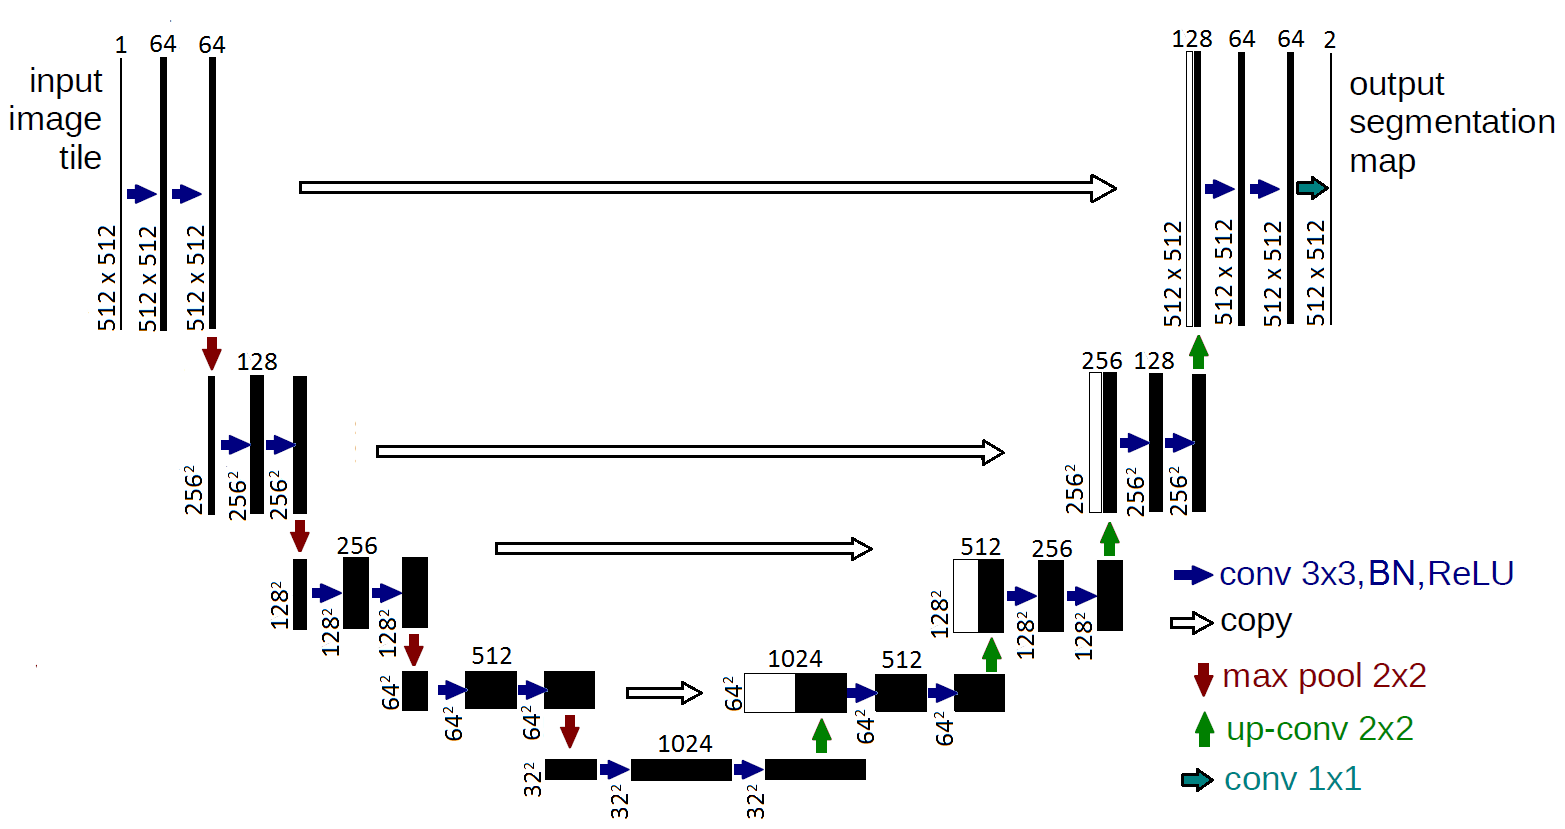
\includegraphics[height=6.0cm]{figures/unet_architecture} 
%\caption{The kidney segmentation FCN based on the UNet architecture. The data is zero-padded to provide full-size segmentation maps, and batch normalization is performed before each activation layer. The figure is adapted from \cite{ronneberger2015u}.}
\caption{The kidney segmentation FCN based on the UNet architecture. The figure is adapted from \cite{ronneberger2015u}.}% The data is zero-padded to provide full-size segmentation maps, and batch normalization is performed before each activation layer. }
\label{fig:unet_arch}
\end{figure}

\section{Data-set}\label{sec:KidSegData}

% SKELETON: Describe the data set used: randomly selected, number of patients/scans, different resolutions, ground truth annotations, heterogeneous data (including sick kidneys with different pathologies).
The data-set for training and evaluating the kidney segmentation algorithm included 46 abdominal CT scans with contrast agent, taken at the portal phase of enhancement. The CT cases were randomly selected within a one-month period and the kidneys were manually annotated by a senior raidiologist. Due to the random selection of the cases, some of them included sick kidneys presenting various pathologies. With the goal of detecting renal lesions in mind, to improve the segmentation robustness to abnormal kidneys, any renal cyst or other pathology observed in the training set was annotated as \emph{kidney} as well. 

\section{Experiments and results}\label{sec:KidSegResults}

% SKELETON: Describe the training process and validation.
The network was trained on  31 scans for 20 epochs with a mini-batch size of 20 images, learning rate of 0.01 for the first 10 epochs and 0.001 for the next 10 epochs, momentum of 0.9 and weight decay of 0.0005. Segmentation accuracy was then evaluated on the remaining 15 CT cases.
Training was performed on an NVIDIA GTX Titan GPU, using the deep learning framework MatConvNet \cite{vedaldi15matconvnet}.

% SKELETON:  Show qualitative and quantitative results.
The accuracy of the 3D segmentation was measured separately for the right and left kidneys in each CT case. Table ~\ref{table:kidSegRes} and Fig.~\ref{fig:kidSegResFull} quantitatively compares between the segmentation results and the ground truth. The network obtained mean dice coefficient of 0.90 for both kidneys.
Qualitative examples of the segmentation output and its comparison to the ground truth labelling are shown in Fig.~\ref{fig:kidSegRes}.
The average running time of kidney segmentation was 51 seconds.

% SKELETON: Table: Segmentation accuracy measurements (recall, precision, Dice coefficient, IOU).
\begin{table}
\centering
\caption{Mean kidney segmentation accuracy evaluated on 15 volumetric CT cases}
\label{table:kidSegRes}
\scalebox{0.9}{
\begin{tabular}{ l | c | c | c | c }
\hline
Organ & Mean recall & Mean precision & Mean IoU & Mean Dice coefficient \\
\hline\hline
Right Kidney & 0.91 $�$ 0.064 & 0.90 $�$ 0.049 & 0.82 $�$ 0.063 & 0.90 $�$ 0.041 \\ \hline
Left Kidney & 0.90 $�$ 0.084 & 0.92 $�$ 0.026 & 0.83 $�$ 0.067 & 0.90 $�$ 0.044 \\ \hline
\end{tabular}
}
\end{table}

\begin{figure}
\centering
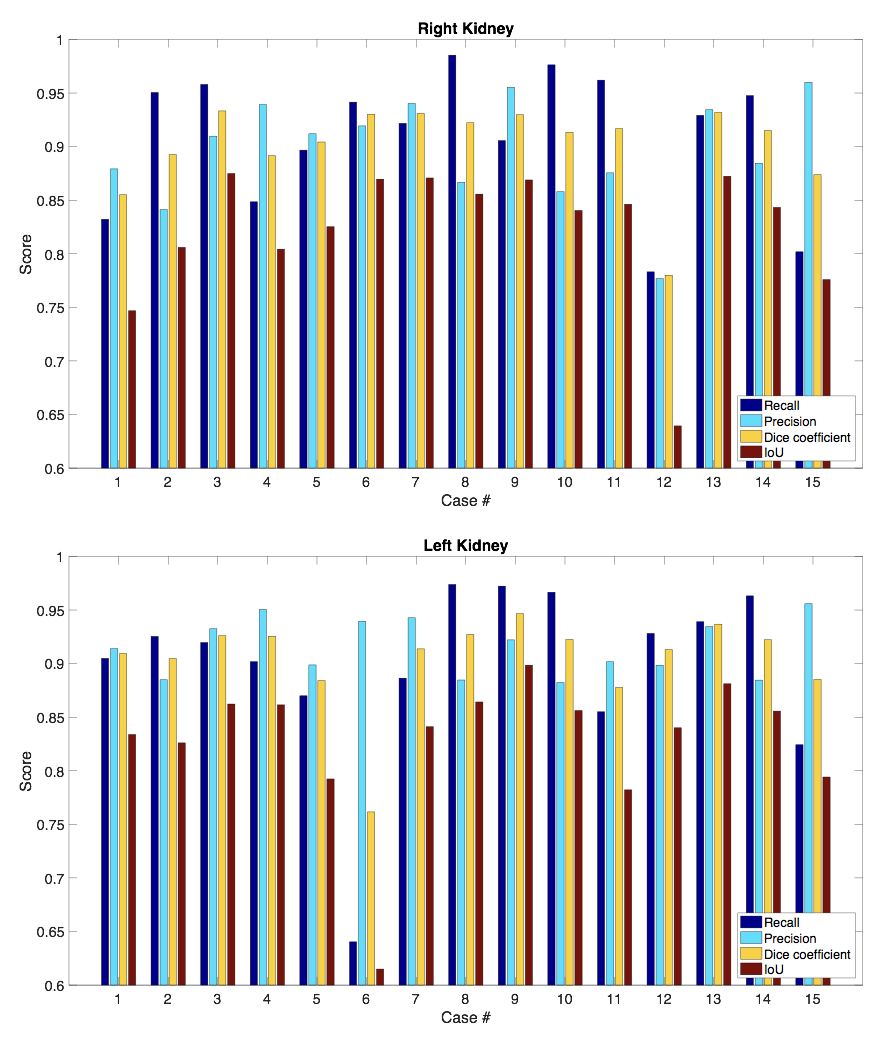
\includegraphics[scale=0.45]{figures/kidney_segmentation_results}
\caption{Kidney segmentation accuracy measurements of 15 volumetric CT cases}
\label{fig:kidSegResFull}
\end{figure}

% SKELETON: Figure: Sample kidney segmentation results in red compared with ground truth annotations in green.
\begin{figure}
\centering
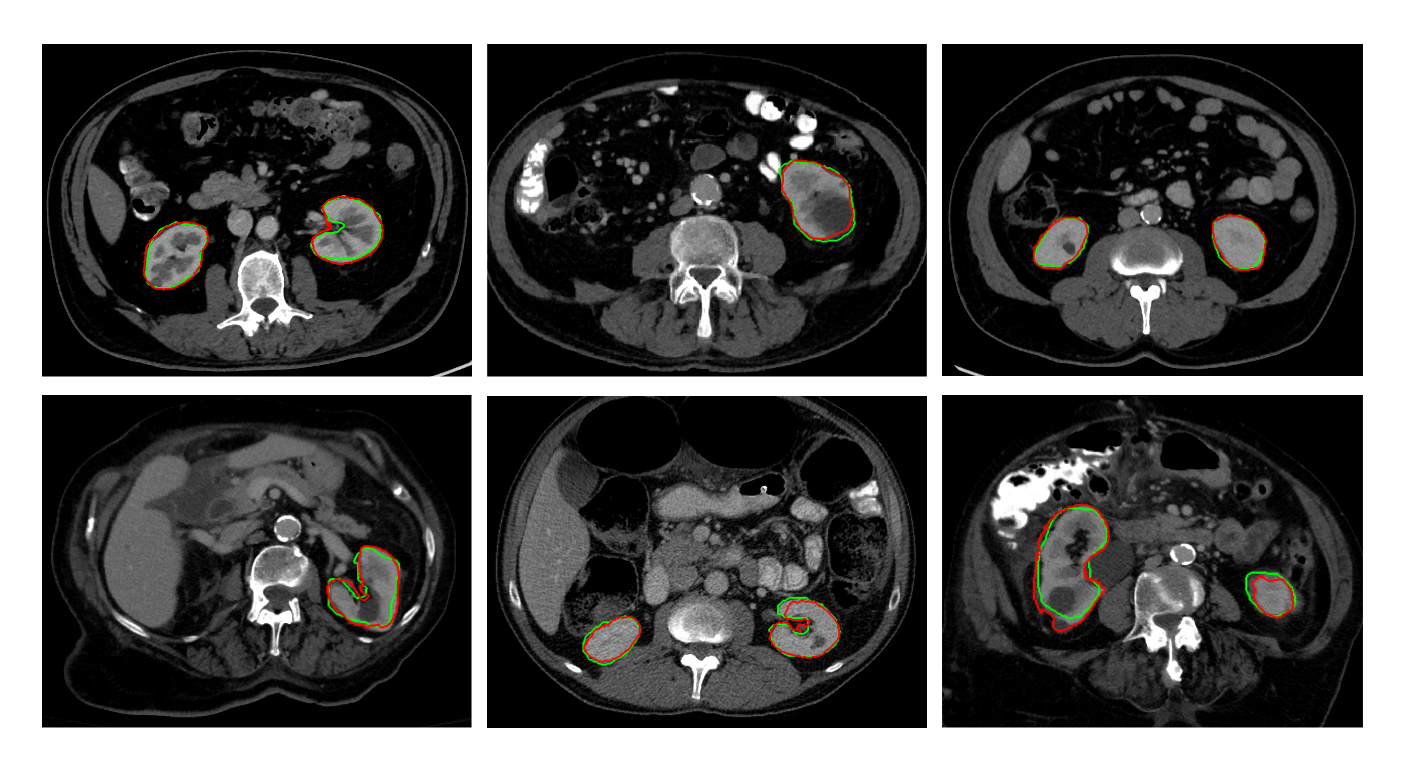
\includegraphics[scale=0.23]{figures/kidney_segmentation}
\caption{Sample kidney segmentation results using the proposed FCN. The manually annotated ground truth (green) and the segmentation map produced by the FCN (red) are marked on the CT images. Simple renal cysts are evident in all of the examples, demonstrating the network's ability to successfully segment them as part of the kidney.}
\label{fig:kidSegRes}
\end{figure}

\section{Discussion}\label{sec:KidSegDiscussion}

% SKELETON: Discuss the results of the kidney segmentation: can they be improved by gathering more data / better quality of ground truth / 3D networks instead of 2D / handling the cyst presence in the ground truth differently.
The kidney segmentation is performed end-to-end by an FCN. Training the network on abdomen CT scans with kidneys presenting multiple cysts and other pathologies achieved promising results, competitive to state-of-the art methods.
% Furthermore, this method proved to be robust and reliable enough for the following step of cyst detection, as will be shown in the next chapter.
When analyzing the segmentation results we noticed that a low recall is often caused by slices in which a renal cyst appears but the kidney is missing. In such cases the cyst was annotated as \emph{kidney} in the ground truth labels but was missed by the FCN. Thus, I believe that the segmentation can be further improved by exploiting 2D slices from all orientations pooled by a majority vote as done in \cite{zhou2016three}, or alternatively, applying a 3D FCN.
It is my opinion that significantly enhanced results can be obtained with the same algorithm, by gathering more data, and by improving the quality of the annotated ground truth.

\chapter{Cyst detection}\label{chapter:CystDetection}

\section{Identification of cyst candidates}\label{sec:CystIdentification}

% SKELETON: Describe the candidate selection algorithm: the input/output, the use of distance maps, and the chosen parameters (thresholding range, minimal radius).
A cyst candidate is the center of a fluid collection,  physically attached to one of the kidneys. To locate cyst candidates we generate two 3D euclidian distance maps by applying a 3D distance transform (DT) \cite{maurer2003linear}. An anisotropic DT is necessary to account for the various scan pixel spacing and spacing between slices. 

In the first map, the value of each voxel is its distance from the closest \emph{non-fluid} voxel, where a fluid voxel is one with HU in the range [-50,80]. As demonstrated in Fig.~\ref{fig:distanceMaps}, \emph{non-fluid} voxels obtain zero value, whereas voxels set in the center of a fluid collection (also referred to as seeds) become regional maxima. For simple renal cysts, which are approximately spherical, the seed's distance to \emph{non-fluid} would be the sphere's radius. We denote the seed's distance to \emph{non-fluid} as $D_{nf}$, and refer to it as the estimated radius of the seed. To reduce the number of potential seeds and considering the scan's resolution, seeds with estimated radius smaller than the spacing between slices are eliminated.
In the second distance map, the value of each voxel is its distance from the closest kidney voxel, denoted $D_k$. We define the adjacency of a seed to the kidney as $D_{nf} - D_k$. For spherical objects, a non-negative adjacency indicates the object and the kidney share a common wall.  A negative value indicates they are separate. Provided with a perfect segmentation of the kidneys, cyst candidates would be seeds with a non-negative adjacency value. However, to account for cases of under-segmentation of the kidneys, we decided to lighthen the adjacency requirement and set the adjacency threshold to 2.5 mm (the spacing between slices).

% SKELETON: Figure: Diagram of the cyst candidate selection flow.
\begin{figure}
\centering
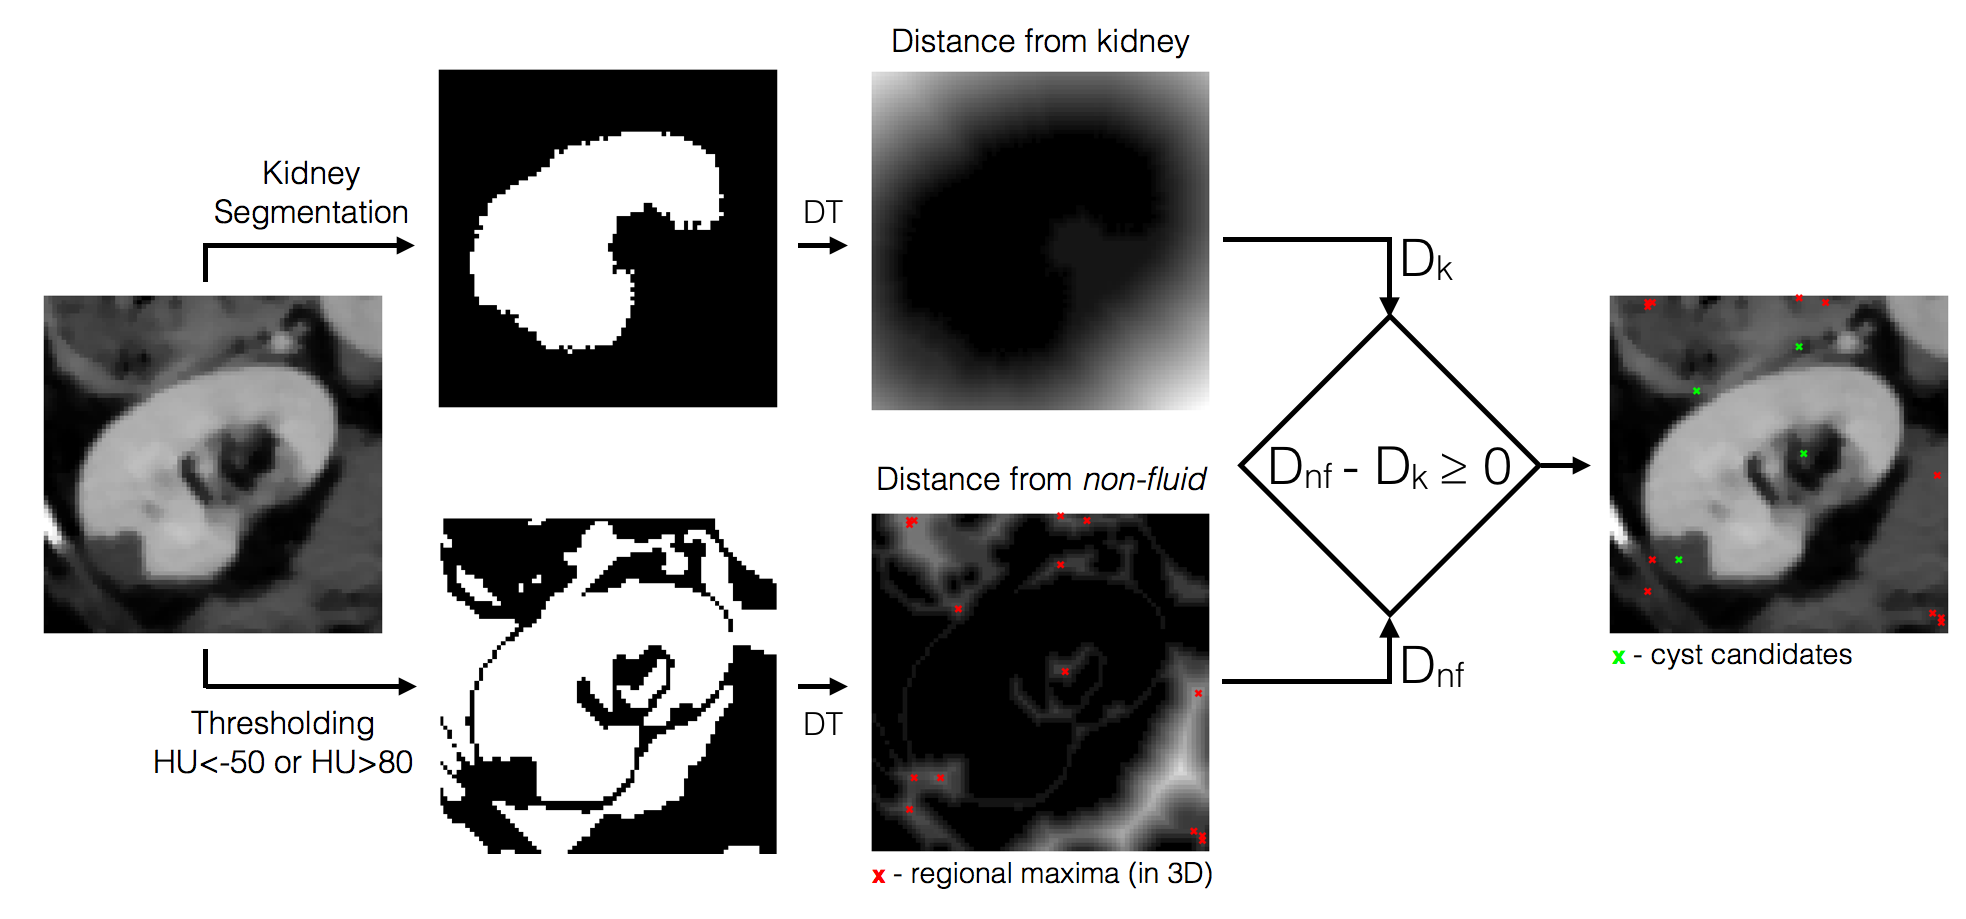
\includegraphics[scale=0.175]{figures/cyst_selection_flow} 
\caption{Main steps of the cyst candidates selection algorithm.}
%An example of renal cysts candidates selection flow. In the upper part of the diagram the kidney is segmented and distance transform (DT) is applied to the result, providing the distance of each voxel from the kidney. In the lower part of the diagram the scan is thresholded to fluids HU range and distance transform is applied to the result, providing the distance of each voxel from the closest \emph{non-fluid} voxel. Regional maxima values (of the 3D distance map) are marked with red X's. Keeping only regional maxima points whose distance from the kidney is smaller than or equal to their distance from \emph{non-fluid} voxels provides us with the selected cysts candidates, marked with green X's.}
\label{fig:distanceMaps}
\end{figure}

\section{Classification of cyst candidates}\label{sec:CystClassification}

% SKELETON: Describe the candidate classification method in detail: the 2.5D patch construction, the data preprocessing (thresholding + Gaussian filter), the network architecture, and the removal of redundant cysts.
Following the detection of cyst candidates, we wish to determine which of them are indeed cysts. We note that the cysts are radially symmetrical and hence their 2D projection has similar properties in any orientation. Capitalizing on this notion, patches of the 2D projections of each candidate on three orthogonal planes (axial, sagittal and coronal) are used to construct a 3-channel image. This representation of a volume-of-interest is known as a 2.5D image \cite{roth2014new}. The patch size is 32x32 pixels and it is sampled from the original CT scan according to the seed's estimated radius so that the suspected object will occupy the central 10x10 pixels of the patch. The sampling is done using bilinear interpolation, after which the patches are smoothed by a gaussian filter ($\sigma=0.5$, kernel size = 3x3) and clipped to HU range [-50,80]. The 2.5D images of the candidates are fed into a small convolutional neural network, composed of three layers of 3x3 convolution and two fully-connected layers, which outputs the probability of each seed being a cyst (see Fig.~\ref{fig:CNNarch}). Seeds with probability greater than 0.5 are classified as cysts.
As a final post-processing step, cysts that are contained in another cyst, i.e. their seed is within the estimated radius of another seed, are considered redundant and eliminated.

% SKELETON: Figure: The cyst classification CNN architecture.
\begin{figure}
\centering
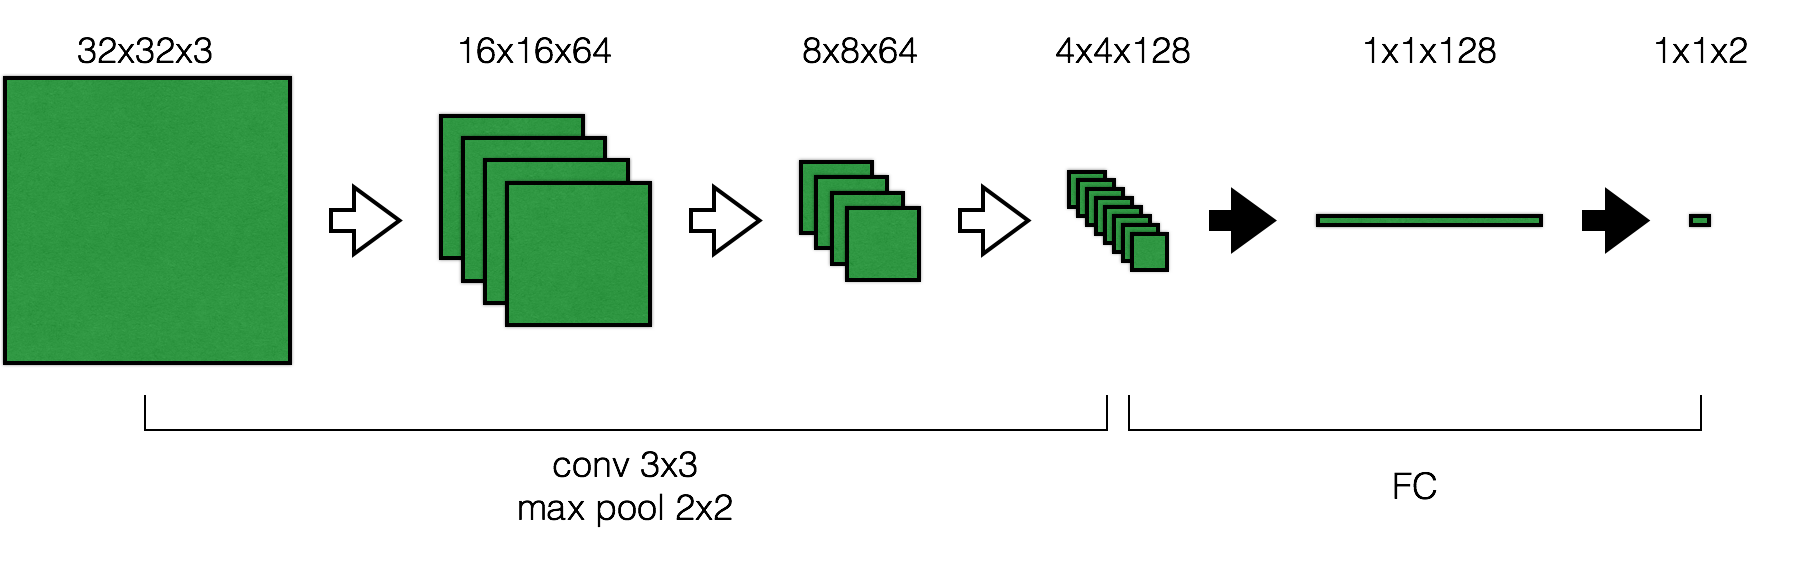
\includegraphics[scale=0.17]{figures/cnn_architecture}
\caption{The cyst classification CNN architecture. The network comprises three layers of 3x3 convolution and 2x2 max pooling followed by two fully-connected (FC) layers.}
\label{fig:CNNarch}
\end{figure}

\section{Data-set}\label{sec:CystData}

% SKELETON: Describe the data-set used: randomly selected, number of patients/scans, number of detected cysts, different resolutions and ground truth annotations.
Our goal was to detect cysts with a diameter of 10 mm or more. A different data-set was used for this task, with 247 such cysts observed in 173 abdominal CT cases. The cases were randomly selected within a one-month period. All scans were taken with contrast agent injection at the portal phase of enhancement, all have a 2.5 mm spacing between slices and pixel spacing of 0.64-0.98 mm. A line was marked along the diameter of each cyst, allowing the extraction of its center and radius.

\section{Experiments and results}\label{sec:CystResults}

% SKELETON: Describe the training process and validation. Show qualitative and quantitative results. Elaborate on the different false-positives that were detected and the false-negatives that were missed. Show that the minimal radius parameter controls the trade-off between TP and TP.
The classification network was trained on a set of ~12,000 seeds extracted from 121 scans for 20 epochs with a mini-batch size of 32 images, learning rate of 0.001 for the first 10 epochs and 0.0001 for the next 10 epochs, momentum of 0.9 and weight decay of 0.001. To increase the number of cysts in the training-set, we augmented the data by rotating and flipping the positive examples. The classification performance was then evaluated on the remaining 52 scans.

The algorithm obtained a true-positive (TP) rate of 83.1\% - 59 out of 71 cysts were successfully detected. Qualitative examples of detected cysts are shown in Fig.~\ref{fig:cysts}. Two cysts were missed due to under-segmentation of the kidney, the rest were incorrectly classified by the network. The algorithm also produced 83 false detections, leading to false-positive rate of 1.6 per patient. However, 5 of these false detections were indications of severe hydronephrosis, still having clinical relevance and requiring radiologist attention. In addition, the algorithm detected 9 more cysts smaller than 10 mm. The average running time of the cyst candidates selection and classification was 22 seconds.

% SKELETON: Figure: Sample cysts detected using the proposed algorithm.
\begin{figure}
\centering
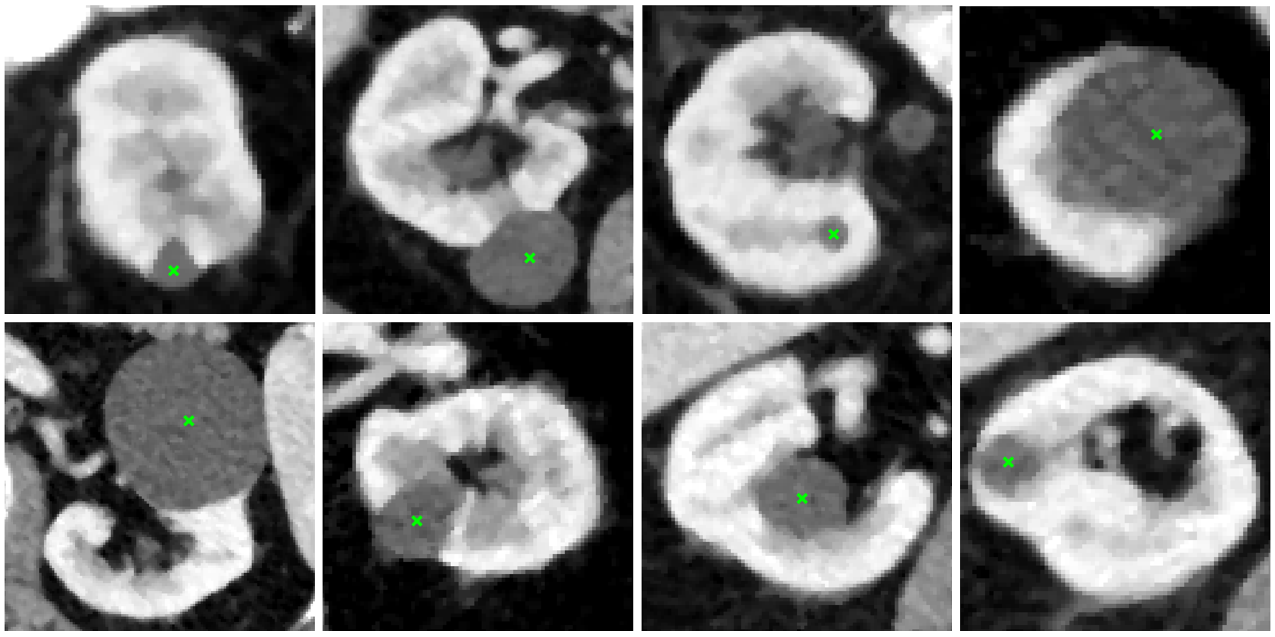
\includegraphics[scale=0.23]{figures/cysts_examples}
\caption{Sample cysts detected using the proposed algorithm.}
\label{fig:cysts}
\end{figure}

In subsection \ref{sec:CystIdentification} we mentioned that seeds with estimated radius less than 2.5 mm are eliminated. The trade-off between the TP and FP rates can be tuned by changing the radius threshold. As shown in Fig.~\ref{fig:ROC} (a), setting the threshold to 3 mm significantly reduces the FP rate from average of 1.6 per patient to 0.88, but at the cost of missing seeds of 4 cysts sized 10-12 mm (5.6\% of the cysts). Reducing the adjacency threshold from 2.5 mm to 0.5 mm leads to a similar result (see Fig.~\ref{fig:ROC} (b)).

% SKELETON: Figure: True-Positives vs. False-Positives (ROC curve) as a function of the minimal radius.
\begin{figure}
\centering
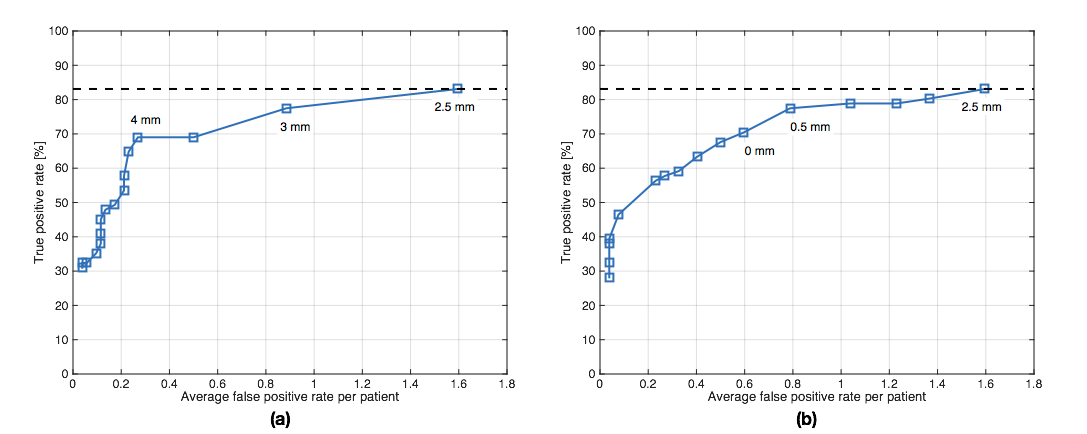
\includegraphics[scale=0.35]{figures/ROC}
\caption{The trade-off between the TP rate and the average FP rate per patient as a function of (a) the radius threshold and (b) the adjacency threshold. The black line is the maximal TP rate that can be achieved on the given data-set with the proposed algorithm.}
\label{fig:ROC}
\end{figure}

\section{Discussion}\label{sec:CystDiscussion}

% SKELETON: Discuss the results of the cyst detection: can they be improved by gathering more data / better quality of ground truth / 3D networks instead of 2D / other approaches (e.g. shape priors).
A combined 3D distance map of the kidneys and surrounding fluids provides us with a large number of cyst candidates (almost 20,000 candidates for 52 scans) but the classification network handles them well, outputting clinically relevant results with high sensitivity and specificity rates. In the context of automatic incidental findings detection, 1.6 FP/case means, in average, less than two unnecessary key image per case. This is an acceptable overhead given the detection benefits of the proposed system. In comparison, Liu et al. reported 15 FP/case computer-aided detection of exophytic renal lesions \cite{liu2015computer}.

The kidney segmentation algorithm proves to be a good start for the purpose of cyst detection. However, a more accurate segmentation would allow us to reduce the adjacency threshold and eliminate a significant amount of the false seeds without missing true cysts. In addition, performing the CT scan with lower spacing between slices would allow us to increase the radius threshold and reduce the false positive rate as well.
While these improvements may eliminate false candidates, the classification network itself is still responsible for the misclassification of 14\% of the cysts. Therefore, improving the network's recall and precision is still a major goal. Training the network with more positive examples and utilizing other augmentations of the data (e.g scaling and noise addition) may help achieve this goal. It is also possible to enrich the data-set by generating synthetic examples using a Generative Adversarial Network.

\chapter{Tumor detection}\label{chapter:TumorDetection}

\section{Data-set}\label{sec:TumorData}
% SKELETON: Describe the data-set used: number of patients/scans with number of detected tumors, different resolutions and ground truth annotations. Show the high variability of the tumors.
After addressing the problem of cyst detection, we approached the challenge of renal tumor detection. Like cysts, tumors vary in size, location and quantity. 
%However, it's the inhomogeneous consistency of the tumors and their undefined shape and borders that make their detection far more complex.
But unlike cysts, tumors have an inhomogeneous consistency and an undefined shape and borders, making their detection and segmentation far more complex. For this task, a data-set of 58 CT cases presenting 58 tumors was used. In each scan the tumor was manually annotated by a senior radiologist. Both kidneys were annotated as well. Fig.~\ref{fig:tumors_var} exhibits the high variability of the tumors in our data-set.
All scans were taken with contrast agent injection at the portal phase of enhancement. The pixel spacing ranges from 0.6836 to 0.9766 mm and the spacing between slices ranges from 1 to 3 mm. 

% Figure: Variability of renal tumors.
\begin{figure}
\centering
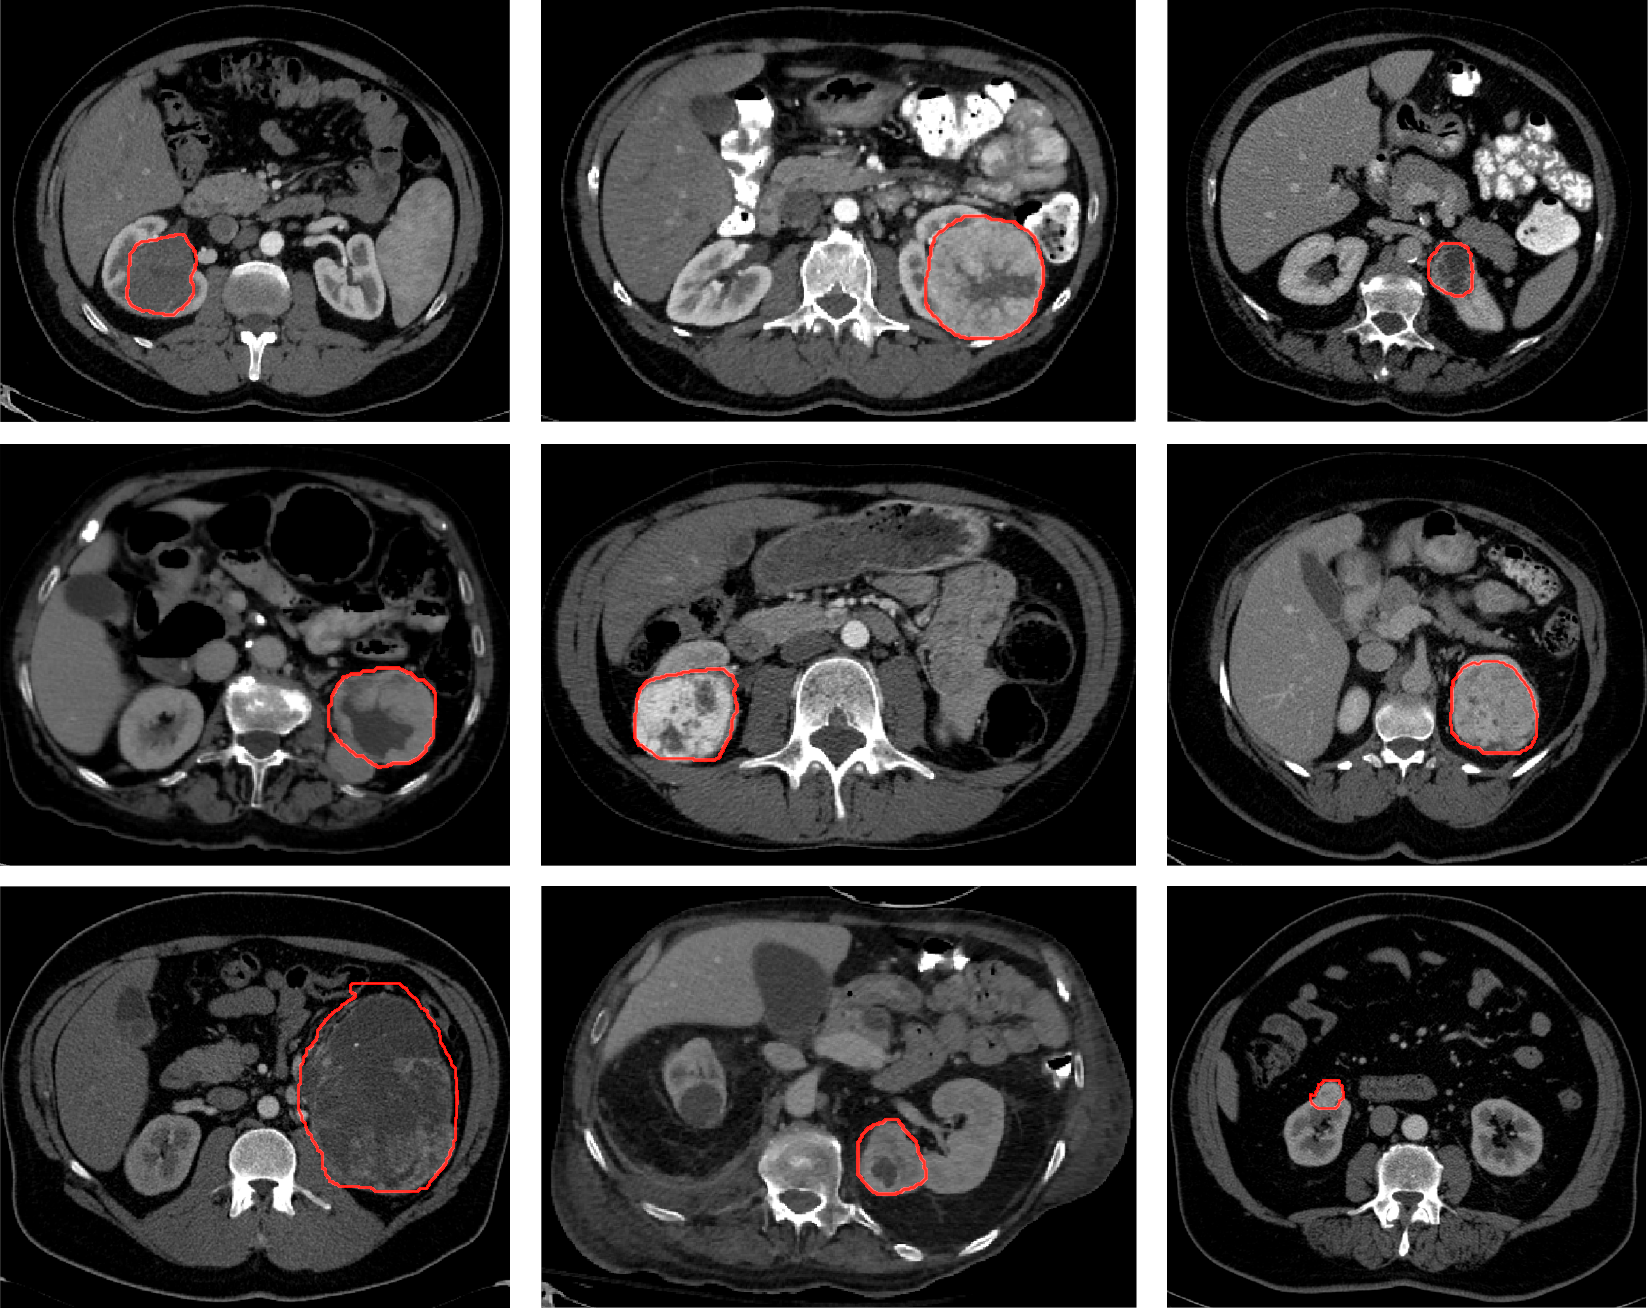
\includegraphics[scale=0.2]{figures/tumors_variability_bold}
\caption{Sample tumors from our data-set demonstrating the high variability of cancerous renal tumors.}
\label{fig:tumors_var}
\end{figure}

\section{Experiments and results}\label{sec:TumorResults}

% SKELETON: Describe different methods and approaches we tried and the unsatisfying results...

Eager/Excited to examine the UNet performance on another segmentation task, we started by training the same architecture to segment tumors in axial 2D slices. We used the exact same parameters as for the kidney segmentation and also the same pre-processing steps. The network learned the training examples pretty well, but the recall and precision on the validation set were low. Moreover, the validation accuracy was not correlated with that of the training set - a clear indication for overfitting.

To handle the overfitting, we tried two approaches. The first approach was to dramatically reduce the capacity of the network. Instead of computing two 3x3 convolutions between the pooling and deconvolution layers, we computed only one, hence cutting the number of parameters almost in half. The results remained practically the same and the problem of overfitting was not resolved. The second approach was to add more data by exploiting 2D slices from all orientations - axial, sagittal and coronal - adding about 10 times more images that include tumors to the data-set. As a result, the recall and precision on the training set improved, but the network's performance on the validation set remained poor. The above-mentioned experiments were conducted using MatConvNet framework, and the results are presented below in Fig.~\ref{fig:tumors_rec_prec}.

\begin{figure}
\centering
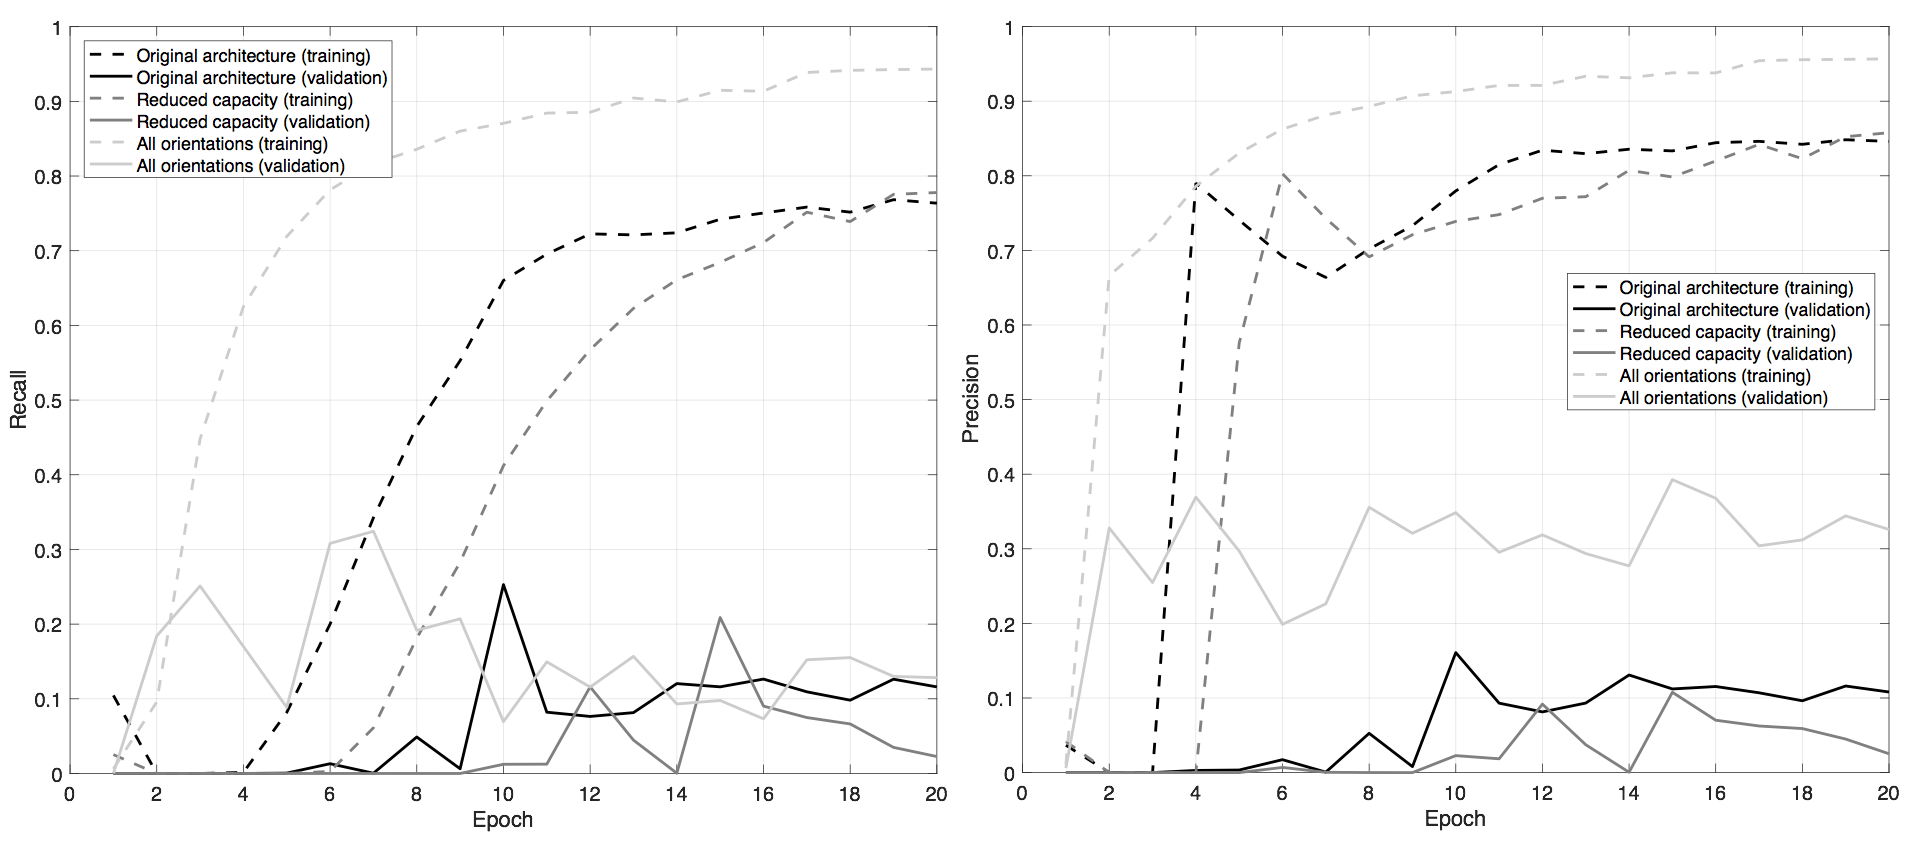
\includegraphics[scale=0.19]{figures/tumors_recall_precision}
\caption{Recall and precision of tumor segmentation on training and validation data-sets using a 2D UNet-based architecture.}
\label{fig:tumors_rec_prec}
\end{figure}

At this point we decided to implement a 3D UNet architecture. Due to memory limitations, we used tensorflow framework \cite{tensorflow2015-whitepaper}. A 3D volume of 128x128x64 voxels was extracted around the center of each kidney and was fed as an input to the 3D network. Since the number of tumor voxels might be very small compared to the volume size, we separated the loss into tumor loss and background loss and tested different linear combinations of the two. The first combination we tested was giving the same weight to the tumor loss and background loss (50-50). The second combination we tested was 20-80, giving lower weight to the tumor loss.
As in our 2D experiments, we clipped the HU of the volumes to the range [-100,400] and normalized them to [-1,1]. We trained the network on 48 kidneys with tumors for 300 epochs with a mini-batch size of 4 volumes. We used Adam optimizer with learning rate of 0.0001. Segmentation accuracy was evaluated at the end of each epoch on the remaining 16 kidneys with tumors. As can be seen in Fig.~\ref{fig:tumors_rec_prec_3D}, when the loss was composed of 20\% tumor loss and 80\% background loss, the learning process seemed promising for the first 100 epochs. From this point on, the performance on the training set continued to improve while the performance on the validation set remained the same and later deteriorated. Meaning, we were not able to overcome the overfitting obstacle by extending the architecture to 3D.

\begin{figure}
\centering
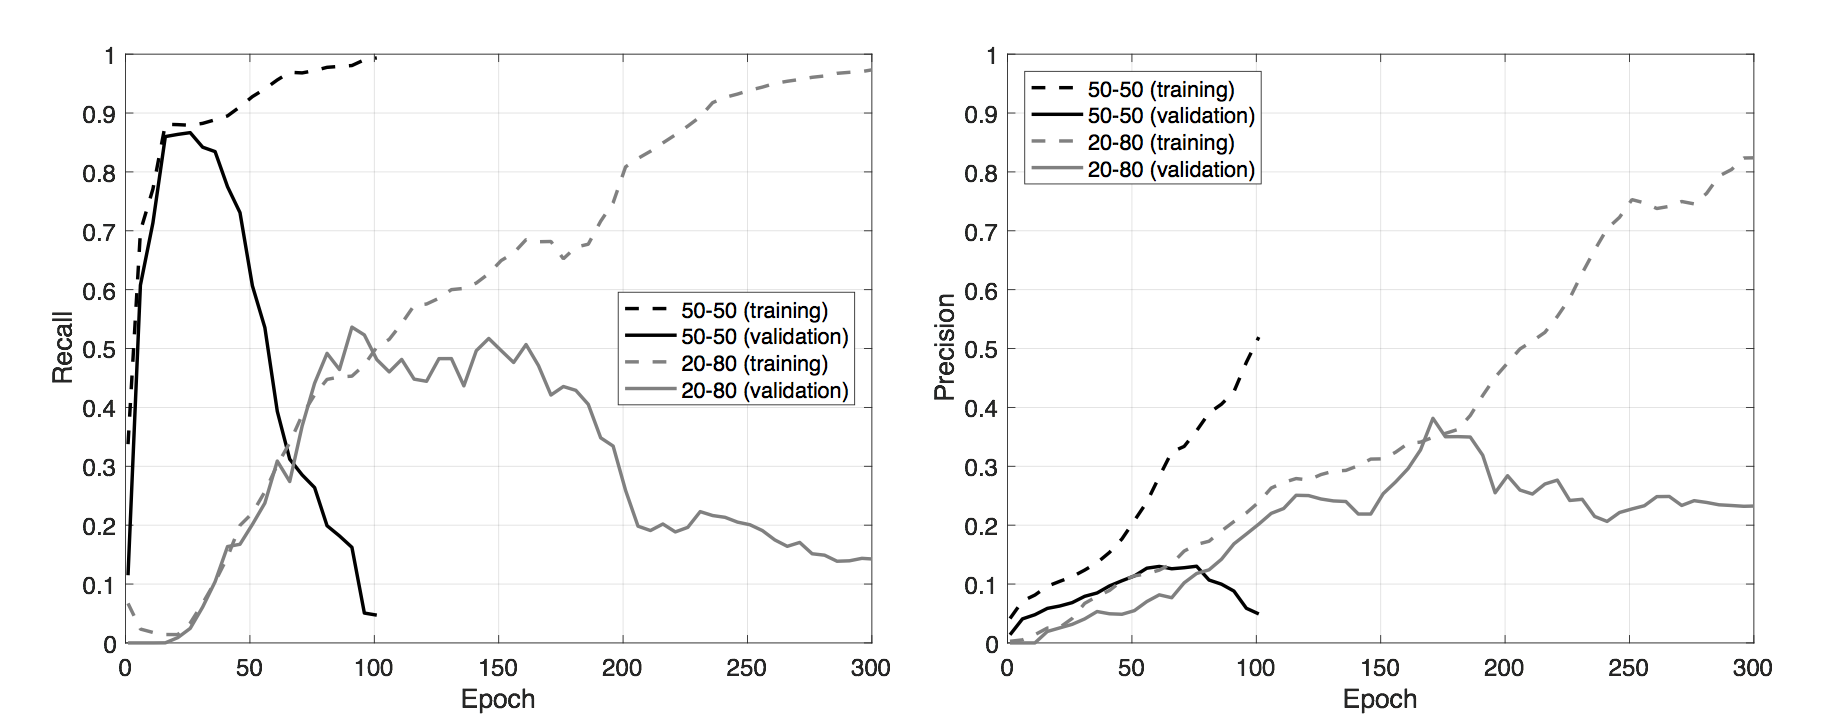
\includegraphics[scale=0.21]{figures/tumors_recall_precision_3D}
\caption{Recall and precision of tumor segmentation on training and validation data-sets using a 3D UNet-based architecture.}
\label{fig:tumors_rec_prec_3D}
\end{figure}

\section{Discussion}\label{sec:TumorDiscussion}

% SKELETON: Discuss the unsolved problem of tumors segmentation - what are we missing? Is it only a matter of gathering more data?
At the beginning of this chapter, in Fig.~\ref{fig:tumors_var}, 9 examples of cancerous renal tumors were presented. These 9 examples account for 15\% of the samples we have, and yet they differ greatly from one another. It is difficult to find one clear and accurate characteristic to describe them all. They are not of the same size, or at the same position, they don't have the same gray-level intensities or the same texture, and they have different shapes and structures. Certainly, we haven't exhausted all research directions regarding detection and segmentation of renal tumors, yet in my opinion it is obvious that our current data-set is not large enough in order to learn from examples. So first and foremost I would recommend to continue collecting more cases to be annotated by the radiologists and perhaps even classified into sub-categories.

To my non-professional eyes, the main common denominator to all examples is the strong deformation of the kidney caused by their presence. In the "lighter" cases, the kidney boundaries become less smooth, or the kidney's homogeneous texture is interrupted. In other cases, the deformation is so severe, making it hard to even recognize that there is a kidney hiding somewhere beneath the tumor. It is often difficult to identify structural changes in the kidney based on a single CT slice, surely if the kidney is not even evident in that slice. Therefore, I think that utilizing a 3D network is worthwhile, and perhaps even essential for the purpose of tumor detection. Same as the doctor usually examines several consecutive slices of the scan together - using a 3D input can provide contextual information that will allow the network to tell where a kidney was supposed to be even if it isn't, and identify the tumor as an anomaly. Of course, causing deformation is not unique to tumors alone, but it can help detect all kinds of lesions. Their classification can then be handled separately.

In my experiments to train the network to segment the tumors, I did not at all use the kidney annotations provided by the radiologist. My naive approach was that if identifying the kidney is essential for detecting renal tumors, then the network will learn to identify kidneys even without their annotations. However, it is possible that learning a separate \emph{kidney} class would have contributed to learning the \emph{tumor} class. Another way to achieve that is to employ transfer-learning and use the kidney segmentation network as a feature extractor or a starting point for the tumor segmentation network. A network that is able to segment kidneys may differentiate between healthy and sick kidney voxels more easily.

One more aspect that is worth discussing, is the network architecture. In my experiments, only the UNet architecture was tested, in 2D and 3D versions. There are many other known architectures that excel in computer vision tasks in general and organ segmentation in medical images in particular. One of these architectures may be more suitable for the task of tumor detection and outperform the UNet. Yet at this point I do not believe that the network architecture is our limitation - the small size of our data-set is.

\chapter{Conclusions}\label{chapter:Conclusions}

% SKELETON: What we did, what we achieved, possible next steps.
We proposed a fully automatic method for kidney segmentation and simple renal cyst detection. Overall, the proposed algorithm is robust and efficient with an average run time of 73 seconds per scan. The algorithm is composed of two separate and independent modules. The first module is responsible for the kidney segmentation. For this purpose we employed an FCN which proved to be suitable for the task. With a larger data-set for training and more accurate annotations, we believe this method could achieve state-of-the-art performance. The kidney segmentation module can provide an infrastructure and a starting point for other automated tools for medical diagnosis of renal diseases.

The second module automatically detects simple renal cysts. It can be easily extended by automatic follow-up, quantification and measurement tools that so far required radiologist intervention for the detection of the cysts. The cyst detection module depends on the kidney segmentation as an input. However, it does not depend on the proposed kidney segmentation module. If another method for kidney segmentation is available, which provides a faster or more accurate segmentation, replacing it would be transparent to the cyst detection module.

We also began exploring the problem of cancerous renal tumor detection, but we were only scratching the surface. Certainly, detecting cancerous tumors is an important objective of high medical relevance. We trained our kidney segmentation network to segment renal tumors, and tested several modifications of the 2D architecture. We tried extending the same architecture to three dimensions as well. All experiments resulted in severe overfitting. These results, along with the visible high variability of the data led us to believe that the data-set must be significantly larger. We still believe that deep convolutional networks may be applicable to this problem, but given the low availability of examples to learn from, devising a more traditional computer vision algorithm might result in more satisfactory detection rates.

\bibliographystyle{plainnat}
\bibliography{references}

\newpage{}

\begin{comment}
It is possible to create the Hebrew part in \LyX{}, but this is less
of our concern. Any typesetting software like \LyX{} (or Word or OpenOffice)
is as good for this purpose. After creating the PDF file from the
Hebrew document, include it here using the Insert -> File -> External
material -> PDFpages (one of the options). See the example below. 
\end{comment}

% TODO: HEBREW PART
% 
\includepdf[pages=-]{hebrew_part}
\end{document}
